\documentclass[11pt]{article}

\usepackage[a4paper,margin=1in]{geometry}
\usepackage[T1]{fontenc}
\usepackage[utf8]{inputenc}
\usepackage{lmodern}
\usepackage{microtype}
\usepackage{amsmath,amssymb,amsthm,mathtools}
\usepackage{booktabs,array}
\usepackage{graphicx}
\usepackage{float}
\usepackage[section]{placeins}
\usepackage{enumitem}
\usepackage[numbers,sort&compress]{natbib}
\usepackage{xcolor}
\usepackage{xurl}
\usepackage[colorlinks=true,linkcolor=blue!55!black,citecolor=blue!55!black,urlcolor=blue!55!black]{hyperref}
\usepackage[nameinlink,noabbrev]{cleveref}

\newtheorem{theorem}{Theorem}[section]
\newtheorem{proposition}[theorem]{Proposition}
\newtheorem{lemma}[theorem]{Lemma}
\newtheorem{corollary}[theorem]{Corollary}
\theoremstyle{definition}
\newtheorem{definition}[theorem]{Definition}
\theoremstyle{remark}
\newtheorem{remark}[theorem]{Remark}

\newcommand{\Id}{I}
\newcommand{\norm}[1]{\left\lVert #1\right\rVert}
\newcommand{\C}{\mathbb C}
\newcommand{\GammaC}{\Gamma}
\newcommand{\eps}{\varepsilon}

\title{Iterated Dyadic Schur Continuation of a Physical Spectral Count\\
\large A Hierarchical Resolvent Certificate from $2048$ to $8192$ Cells\\
at a Quadratic Band-Merging Map}
\author{Liang Wang}
\date{July 2026}

\begin{document}
\maketitle

\begin{abstract}
A preceding computer-assisted theorem proved that exact stored
Perron/parity-extracted physical two-step matrices on $2048$ and $4096$
midpoint cells each have one eigenvalue inside a prescribed complex circle.
Its direct coarse resolvent atlas did not by itself provide an efficient route
to the next grid.  We give a second rigorous dyadic continuation, at fixed
Gaussian width \(\sigma=10^{-2}\), and introduce a hierarchical resolvent
estimate that avoids a direct $4096$-dimensional inverse atlas.

For the $4096\to8192$ split, componentwise outward residuals around four
rank-$96$ centers certify the coarse-consistency, coarse-to-detail,
detail-to-coarse, and detail blocks by

\[
4.97036\times10^{-5},\quad 5.66125\times10^{-3},\quad
6.86176\times10^{-3},\quad 3.26337\times10^{-5}.
\]

The resulting second-level effective perturbation is at most
$1.52962\times10^{-4}$, so an $A_{4096}$ resolvent bound below
$6537.58$ is sufficient.  We tighten the inherited $A_{2048}$ atlas from
170 to 183 rigorous centers and form an exact 324-leaf rational contour
partition.  An exact Schur block-inverse formula propagates each leafwise
$A_{2048}$ bound through the first refinement.  The worst propagated
$A_{4096}$ resolvent is $4843.82$, and the final matrix Rouch\'e product is
$0.740919<1$.  Hence, for the exact archived binary64 matrices,

\[
 \boxed{N_{\Gamma}(A_{2048})=N_{\Gamma}(A_{4096})
 =N_{\Gamma}(A_{8192})=1.}
\]

This is a finite stored-matrix theorem at one noise scale.  It does not prove
a continuum limit, an all-dimensions induction, a zero-noise limit, a zeta-zero
identification, a Hilbert--P\'olya construction, or the Riemann hypothesis.
\end{abstract}

\section{Introduction}

The previous nested-grid certificate \citep{WangNested2026} answered one
discretization-stability question: a contour count proved at dimension $2048$
survives the refinement to $4096$.  Repeating that proof naively at the next
scale would require a direct atlas of rigorous inverses for a
$4096$-dimensional nonnormal matrix.  Such an atlas is possible in principle,
but it discards the exact coarse/detail structure already certified at the
first refinement.

This paper asks a sharper question.  Can the first Schur decomposition be
used not only to transfer a count, but also to transfer a \emph{resolvent
bound} strong enough to close the next count comparison?  The answer is yes
for the exact stored matrices studied here.  The proof chain is

\[
\begin{gathered}
\text{direct }A_{2048}\text{ resolvent centers}
\longrightarrow
\text{first Schur effective inverse}
\longrightarrow
\text{full }A_{4096}\text{ resolvent}\notag\\
\longrightarrow
\text{second Schur effective comparison}
\longrightarrow
N_{\Gamma}(A_{8192})=N_{\Gamma}(A_{4096}).
\end{gathered}
\]

The distinction matters because these transfer matrices are strongly
nonnormal.  Eigenvalue displacements alone do not control contour counts;
resolvent amplification is the relevant quantity
\citep{Kato1995,TrefethenEmbree2005}.  The new estimate keeps that amplification
visible at both refinement levels.

The principal contributions are as follows.

\begin{enumerate}[leftmargin=2em]
 \item We certify the exact $4096\to8192$ coarse/detail blocks by
       componentwise factor-graph residuals.  Relative to the first split,
       the two consistency/detail blocks are approximately one quarter as
       large and the cross channels approximately one half as large.
 \item We prove a norm-preserving block-inverse propagation formula.  It turns
       a leafwise $A_{2048}$ resolvent upper $M_0$ into a rigorous
       $A_{4096}$ upper without constructing a $4096$-dimensional inverse.
 \item We tighten the inherited direct atlas with only 13 additional centers.
       The resulting exact rational partition closes both the first effective
       inverse gate and the second matrix Rouch\'e gate.
 \item We bitwise identify the $A_{4096}$ factor object used here with the
       one certified in the preceding theorem, thereby obtaining the
       three-scale count chain.
\end{enumerate}

The observed scaling is encouraging, but this paper does not promote two
finite ratios to an asymptotic law.  An induction would require uniform block
estimates and a uniformly controlled hierarchical resolvent atlas, neither of
which is proved here.

\section{Stored matrices, contour, and inherited count}
\label{sec:objects}

Let $P_m$ be the archived row-normalized folded Gaussian midpoint matrix on
$m$ positive cells.  Let

\[
X_m,Y_m\in\mathbb R^{m\times2},\qquad
\Lambda_m\in\mathbb R^{2\times2}
\]

be the stored right modes, left modes, and peripheral eigenvalue diagonal.
The Perron/parity-extracted one-step and physical two-step matrices are

\begin{equation}
 U_m=P_m-X_m\Lambda_mY_m^T,
 \qquad A_m=U_m^2.
 \label{eq:physical}
\end{equation}

Every binary64 entry in these factors is treated as an exact real number.  We
write

\[
A_0=A_{2048},\qquad A_1=A_{4096},\qquad A_2=A_{8192}.
\]

The positively oriented counting circle is

\begin{equation}
 \GammaC:\quad z=z_0+r e^{i\theta},\qquad 0\le\theta\le2\pi,
 \label{eq:contour}
\end{equation}

with stored values

\begin{equation}
 z_0=-0.3233504401504541-0.5508412474453575i,
 \qquad r=0.2624987592858511.
 \label{eq:contour-values}
\end{equation}

The distance from the origin to the closed counting disk satisfies

\begin{equation}
 \rho_0=|z_0|-r\ge0.376235604149098.
 \label{eq:origin-distance}
\end{equation}

For a matrix $A$, let $N_{\Gamma}(A)$ denote the algebraic number of
eigenvalues in the interior of \(\Gamma\).

\begin{proposition}[Inherited stored count]
\label{prop:inherited}
For the exact archived factors at \(\sigma=10^{-2}\),

\[
N_{\Gamma}(A_0)=N_{\Gamma}(A_1)=1.
\]

The $A_1$ sparse matrix, right and left peripheral modes, and peripheral
values consumed in the present snapshot are bitwise identical to those in
the preceding certificate.
\end{proposition}

\begin{proof}
The count is the main theorem of \citet{WangNested2026}, built on the exact
packet-pair count of \citet{WangPacketPair2026}.  The present replay hashes the
sparse data, indices, row pointers, right modes, left modes, and peripheral
values independently.  All six hashes agree with the inherited $A_1$
object, and the inherited snapshot and theorem hashes also agree with the
archive.
\end{proof}

We distinguish exact algebra, rigorous stored-binary64 certificates, and
floating diagnostics.  Only the first two enter the theorem.  Sparse
eigensolves are reported later solely to localize the counted eigenvalue.

\section{Exact dyadic coordinates at two levels}
\label{sec:coordinates}

For a dyadic refinement from $n$ to $2n$, define replication and
alternating-detail injections by

\[
(Jx)_{2k}=(Jx)_{2k+1}=x_k,
\qquad
(Ky)_{2k}=y_k,\quad (Ky)_{2k+1}=-y_k.
\]

Define the corresponding restrictions

\[
R=\frac12J^T,\qquad S=\frac12K^T,
\]

and set

\[
T=[J\ K],\qquad T^{-1}=\begin{bmatrix}R\\S\end{bmatrix}.
\]

These identities are exact over the stored reals.  Moreover
$T=\sqrt2\,Q$ for an orthogonal $Q$, so

\begin{equation}
 T^{-1}MT=Q^TMQ,\qquad \norm{T^{-1}MT}_2=\norm{M}_2.
 \label{eq:norm-invariance}
\end{equation}

Thus the unnormalized integer-valued coordinate maps introduce no condition
number loss in the Euclidean norm.

At refinement level $j=1,2$, the exact coordinate block form is

\begin{equation}
 T_j^{-1}A_jT_j=
 \begin{pmatrix}
 A_{j-1}+E_j & B_j\\
 C_j & D_j
 \end{pmatrix}.
 \label{eq:block-form}
\end{equation}

Here $C_j$ maps coarse coordinates to detail coordinates, while $B_j$
maps detail coordinates back to coarse coordinates.  Whenever
$z-D_j$ is invertible, define

\begin{align}
 R_{D,j}(z)&=(z-D_j)^{-1},\label{eq:detail-resolvent}\\
 \Delta_j(z)&=E_j+B_jR_{D,j}(z)C_j,\label{eq:self-energy}\\
 F_j(z)&=z-A_{j-1}-\Delta_j(z).\label{eq:effective}
\end{align}

The exact Schur determinant identity is

\begin{equation}
 \det(z-A_j)=\det(z-D_j)\det F_j(z).
 \label{eq:schur-determinant}
\end{equation}

If \(\norm{D_j}_2<\rho_0\), every eigenvalue of $D_j$ lies in the
origin-centered disk of radius \(\norm{D_j}_2\), which is disjoint from the
counting disk.  In that case

\begin{equation}
 \sup_{z\in\Gamma}\norm{R_{D,j}(z)}_2
 \le d_j:=\frac{1}{\rho_0-\norm{D_j}_2},
 \label{eq:detail-bound}
\end{equation}

and

\begin{equation}
 \sup_{z\in\Gamma}\norm{\Delta_j(z)}_2
 \le \eps_j:=\norm{E_j}_2+
 \norm{B_j}_2d_j\norm{C_j}_2.
 \label{eq:epsilon}
\end{equation}

\section{Certified second-level block bounds}
\label{sec:blocks}

The proof objects for each block are stored rank-$96$ factors
$L\Sigma V^T$.  They are not assumed exact singular decompositions.  The
following elementary estimate explains how they enter the certificate.

\begin{lemma}[Low-rank center plus full residual]
\label{lem:low-rank}
Let $H$ be an exact stored block, and let $L,\Sigma,V$ be stored factors.
If

\[
\norm{L^TL-I}_F\le\delta_L,
\qquad
\norm{V^TV-I}_F\le\delta_V,
\]

then

\begin{equation}
 \norm{H}_2\le
 \sqrt{1+\delta_L}\,\norm{\Sigma}_2\sqrt{1+\delta_V}
 +\norm{H-L\Sigma V^T}_F.
 \label{eq:low-rank-bound}
\end{equation}
\end{lemma}

\begin{proof}
The Gram estimates imply
$\norm{L}_2\le\sqrt{1+\delta_L}$ and
$\norm{V}_2\le\sqrt{1+\delta_V}$.  Apply the triangle inequality,
submultiplicativity, and \(\norm{R}_2\le\norm{R}_F\).
\end{proof}

Every matrix action used to form the residual in
\eqref{eq:low-rank-bound} is evaluated by componentwise outward arithmetic.
The reported Frobenius residual contains both the residual center and its
complete radius.  Standard verified-floating-point principles are described
in \citet{Higham2002,Rump2010}; the factor-graph implementation is inherited
from \citet{WangOutwardCode2026}.

\begin{table}[H]
\centering
\caption{Certified block norms at the two dyadic levels.  The last column is
the full second-level Frobenius residual after subtracting the stored
rank-$96$ center.}
\label{tab:blocks}
\begin{tabular}{lrrrr}
\toprule
block & first-level upper & second-level upper & ratio & second residual\\
\midrule
$E$ & $1.98877177\!\times10^{-4}$ & $4.97035044\!\times10^{-5}$ & $0.249921$ & $7.4855\!\times10^{-10}$\\
$C$ & $1.13214379\!\times10^{-2}$ & $5.66124305\!\times10^{-3}$ & $0.500046$ & $1.5175\!\times10^{-8}$\\
$B$ & $1.37226417\!\times10^{-2}$ & $6.86175172\!\times10^{-3}$ & $0.500031$ & $7.1604\!\times10^{-9}$\\
$D$ & $1.30522077\!\times10^{-4}$ & $3.26336986\!\times10^{-5}$ & $0.250024$ & $3.3016\!\times10^{-10}$\\
\bottomrule
\end{tabular}
\end{table}

For the second split, \eqref{eq:detail-bound} gives

\begin{equation}
 d_2\le2.658139564401696.
 \label{eq:d2}
\end{equation}

The second Schur self-energy and total effective perturbation satisfy

\begin{align}
 \norm{B_2}_2d_2\norm{C_2}_2
 &\le1.0325820704184003\times10^{-4},\label{eq:self2}\\
 \eps_2
 &\le1.5296171140743076\times10^{-4}.
 \label{eq:epsilon2}
\end{align}

Consequently, a contour-wide $A_1$ resolvent bound below

\begin{equation}
 \eps_2^{-1}\ge6537.583757391333
 \label{eq:second-threshold}
\end{equation}

is sufficient for the second matrix Rouch\'e comparison.

\section{Hierarchical propagation of the 4096-dimensional resolvent}
\label{sec:propagation}

The threshold in \eqref{eq:second-threshold} could be tested by direct
$4096$-dimensional inverse certificates.  Instead we propagate the existing
direct $A_0$ atlas through the first exact block decomposition.

\begin{proposition}[Schur resolvent propagation]
\label{prop:resolvent-propagation}
Fix $z\in\Gamma$.  Suppose

\[
\norm{(z-A_0)^{-1}}_2\le M_0,
\qquad M_0\eps_1<1.
\]

Let $d_1$ be the first detail-resolvent upper from
\eqref{eq:detail-bound}.  Then

\begin{equation}
\begin{split}
 \norm{(z-A_1)^{-1}}_2
 \le M_1(M_0):={}&d_1\\
 &+\sqrt{1+(d_1\norm{C_1}_2)^2}
 \sqrt{1+(d_1\norm{B_1}_2)^2}
 \frac{M_0}{1-M_0\eps_1}.
\end{split}
\label{eq:propagated-bound}
\end{equation}
\end{proposition}

\begin{proof}
Write $R_0=(z-A_0)^{-1}$.  By
\eqref{eq:self-energy}--\eqref{eq:effective},

\[
F_1=(z-A_0)\bigl(I-R_0\Delta_1(z)\bigr).
\]

The Neumann bound gives

\begin{equation}
 \norm{F_1^{-1}}_2\le\frac{M_0}{1-M_0\eps_1}.
 \label{eq:effective-inverse-bound}
\end{equation}

The exact inverse of the first block matrix factors as

\begin{equation}
\begin{split}
 &\left(
 z-\begin{pmatrix}A_0+E_1&B_1\\C_1&D_1\end{pmatrix}
 \right)^{-1}\\
 &\qquad=
 \begin{bmatrix}I\\R_{D,1}C_1\end{bmatrix}
 F_1^{-1}
 \begin{bmatrix}I&B_1R_{D,1}\end{bmatrix}
 +\begin{pmatrix}0&0\\0&R_{D,1}\end{pmatrix}.
\end{split}
\label{eq:block-inverse}
\end{equation}

The column and row graph factors obey

\[
\left\|\begin{bmatrix}I\\R_{D,1}C_1\end{bmatrix}\right\|_2
\le\sqrt{1+(d_1\norm{C_1}_2)^2},
\]

\[
\left\|\begin{bmatrix}I&B_1R_{D,1}\end{bmatrix}\right\|_2
\le\sqrt{1+(d_1\norm{B_1}_2)^2}.
\]

Combine these estimates with \eqref{eq:effective-inverse-bound}.  Finally,
\eqref{eq:norm-invariance} identifies the coordinate-space norm with the
ambient $A_1$ resolvent norm.
\end{proof}

The first-level certificate supplies

\begin{equation}
 d_1\le2.658831394912469,
 \qquad
 \eps_1\le6.119533154024968\times10^{-4}.
 \label{eq:first-constants}
\end{equation}

The two graph factors in \eqref{eq:propagated-bound} are bounded by

\[
1.000452956430038,\qquad1.000665399669618.
\]

Thus the only remaining task is a sufficiently tight leafwise bound for the
direct $A_0$ resolvent.

\section{A tightened direct atlas and two simultaneous gates}
\label{sec:atlas}

At a rigorous direct center \(\zeta\), let

\[
\norm{(\zeta-A_0)^{-1}}_2\le M_\zeta.
\]

For a circular-arc enclosure contained in a disk satisfying
$M_\zeta\delta<1$, the resolvent identity yields

\begin{equation}
 \sup_{|z-\zeta|\le\delta}\norm{(z-A_0)^{-1}}_2
 \le\frac{M_\zeta}{1-M_\zeta\delta}.
 \label{eq:center-transport}
\end{equation}

The inherited archive contains 170 such centers.  We request the stronger
first-level target

\begin{equation}
 M_0\eps_1<0.75,
 \qquad
 M_0<\frac{0.75}{\eps_1}=1225.583686080214\ldots.
 \label{eq:tight-target}
\end{equation}

Only 13 additional direct centers are needed.  Adaptive exact bisection then
produces 324 rational leaves, with maximum refinement level eight and no
unresolved component.  The leaves form an exact partition of one contour
turn.

\begin{table}[H]
\centering
\caption{Outward-rounded maxima over the exact 324-leaf propagated atlas.}
\label{tab:atlas}
\begin{tabular}{lr}
\toprule
quantity & certified upper\\
\midrule
transported $A_0$ resolvent $M_0$ & $1221.3793571000042$\\
first effective product $M_0\eps_1$ & $0.7474271469415178$\\
first effective inverse $\norm{F_1^{-1}}_2$ & $4835.750724236383$\\
propagated $A_1$ resolvent $M_1$ & $4843.819104431207$\\
second continuation product $M_1\eps_2$ & $0.7409188599618061$\\
\bottomrule
\end{tabular}
\end{table}

Both products are evaluated leaf by leaf; the maxima need not occur on the
same leaf.  In particular, the final value in \cref{tab:atlas} lies well below
one and the propagated $A_1$ bound lies below the independent threshold in
\eqref{eq:second-threshold}.

\section{The certified three-scale count}
\label{sec:theorem}

We use the finite-dimensional analytic matrix form of Rouch\'e's theorem
\citep{Ahlfors1979,GohbergSigal1971}.  If $A(z)$ is invertible on
\(\Gamma\), $B(z)$ is analytic on and inside the contour, and

\[
\sup_{z\in\Gamma}\norm{A(z)^{-1}B(z)}_2<1,
\]

then $A$ and $A+B$ have the same determinant zero count inside the
contour.

\begin{theorem}[Certified iterated dyadic physical count]
\label{thm:main}
At \(\sigma=10^{-2}\), for the exact stored binary64 physical two-step
matrices defined in \eqref{eq:physical},

\[
\boxed{N_{\Gamma}(A_{2048})=N_{\Gamma}(A_{4096})
=N_{\Gamma}(A_{8192})=1.}
\]
\end{theorem}

\begin{proof}
By \cref{prop:inherited}, $N_{\Gamma}(A_1)=1$.  The second detail block
satisfies

\[
\norm{D_2}_2\le3.2633698567\times10^{-5}<\rho_0,
\]

so $z-D_2$ is invertible on and inside the counting disk and
$N_{\Gamma}(D_2)=0$.  Hence \(\Delta_2(z)\) is analytic there.

On every leaf, \cref{prop:resolvent-propagation} and the direct center
transport \eqref{eq:center-transport} give a rigorous bound for
$(z-A_1)^{-1}$.  The exact rational partition covers all of \(\Gamma\), and
\cref{tab:atlas} gives

\[
\sup_{z\in\Gamma}
\norm{(z-A_1)^{-1}\Delta_2(z)}_2
\le0.7409188599618061<1.
\]

Matrix Rouch\'e therefore shows that

\[
N_{\Gamma}(F_2)=N_{\Gamma}(z-A_1)=1.
\]

The exact determinant factorization \eqref{eq:schur-determinant} yields

\[
N_{\Gamma}(A_2)=N_{\Gamma}(D_2)+N_{\Gamma}(F_2)=0+1=1.
\]

Combining this with the inherited count proves the stated chain.
\end{proof}

\section{Finite-scale diagnostics and what they do not prove}
\label{sec:diagnostics}

\begin{figure}[H]
\centering
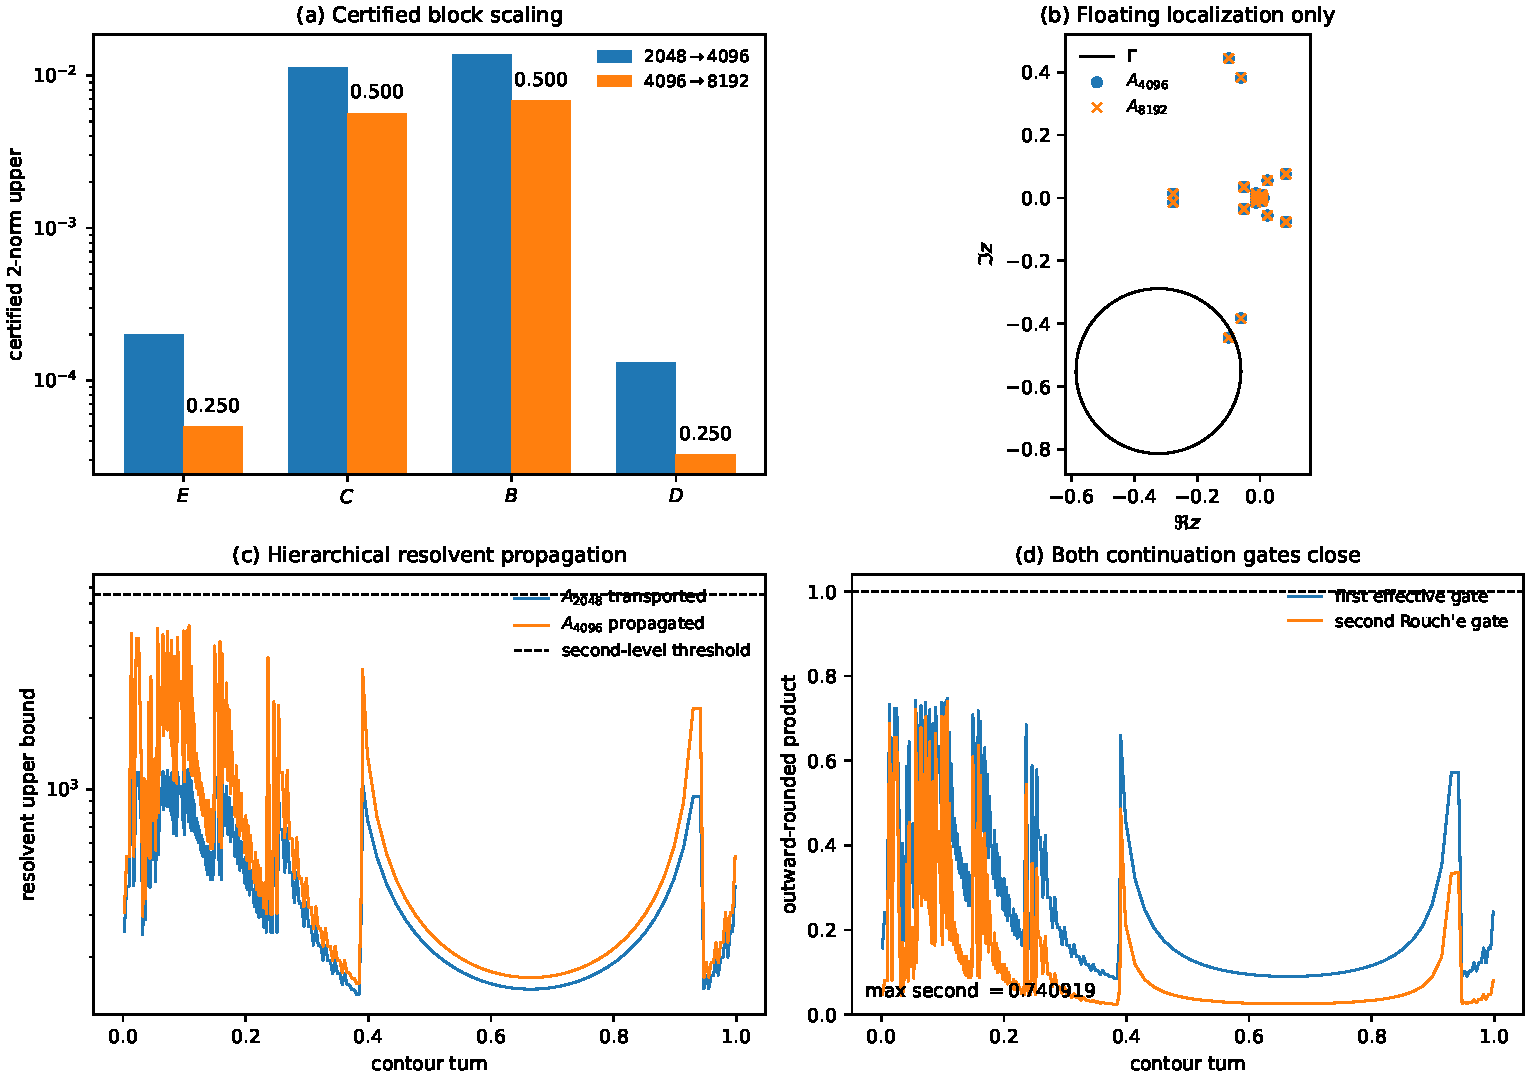
\includegraphics[width=\textwidth]{figures/iterated_dyadic_physical_count.pdf}
\caption{Second dyadic continuation diagnostics and certificates.  (a) The
second certified consistency and detail blocks are approximately one quarter
of the first-level bounds, while the cross channels are approximately one
half.  (b) Floating sparse eigenvalues are shown only for localization; the
count theorem does not use them.  (c) The direct $A_{2048}$ leaf bounds are
propagated to $A_{4096}$ by \eqref{eq:propagated-bound}, remaining below the
second-level threshold.  (d) Both outward-rounded continuation products stay
below one.}
\label{fig:summary}
\end{figure}

The floating pilot resolves one eigenvalue inside \(\Gamma\) at each of the
two larger dimensions.  Their approximate locations are

\[
-0.0994035212675-0.4441920040123i
\]

and

\[
-0.0994142875185-0.4441895651018i,
\]

with displacement $1.10391\times10^{-5}$.  Residuals are below
$1.3\times10^{-15}$.  These values help visualize the theorem but do not
certify the count.

The second-to-first block ratios are

\[
0.249921,\quad0.500046,\quad0.500031,\quad0.250024.
\]

The self-energy and full effective perturbation ratios are respectively
$0.249974$ and $0.249957$.  This is consistent with a first-order decay of
cross channels and a second-order decay of consistency/detail errors under one
additional dyadic refinement.  It is evidence for a possible multilevel
estimate, not a proof of one.  A genuine induction would have to control:

\begin{enumerate}[leftmargin=2em]
 \item the block ratios uniformly over all sufficiently fine grids;
 \item the growth of the recursively propagated nonnormal resolvent;
 \item the number and quality of direct base-grid centers needed to cover the
       full contour; and
 \item the relation of the stored finite matrices to a continuum operator.
\end{enumerate}

The present theorem closes one additional finite level and isolates these
remaining obstructions quantitatively.

\section{Archive and reproducibility}
\label{sec:archive}

The archive separates proof inputs from diagnostics.

\begin{itemize}[leftmargin=2em]
 \item The exact $A_{8192}$ sparse factor object is stored separately from
       four rank-$96$ center archives.  Every file is below the repository's
       single-file limit.  The hash of the original monolithic construction
       snapshot and every constituent array hash are retained.
 \item The second block certificate records factor Gram defects, singular
       scale uppers, full residual Frobenius uppers, and residual hashes.
 \item The direct center archive contains 170 inherited and 13 additional
       rigorous $A_{2048}$ center bounds.
 \item The 324-leaf CSV ledger records exact rational endpoints, center
       transport data, first effective products, propagated $A_{4096}$
       bounds, and second continuation products.
 \item A final JSON certificate composes object identity, detail exclusion,
       inherited count, exact partition, and both Rouch\'e gates.
\end{itemize}

The fast verification sequence is

\begin{verbatim}
python -m pytest -q -p no:cacheprovider
python experiments/build_final_certificate.py
python experiments/build_archive.py
MPLBACKEND=Agg python experiments/make_figures.py
latexmk -pdf -interaction=nonstopmode -halt-on-error main.tex
cp main.pdf iterated-dyadic-physical-count.pdf
python experiments/verify_archive.py
\end{verbatim}

Recomputing the componentwise second-level residual certificate is the most
expensive replay step.  It is run by

\begin{verbatim}
OPENBLAS_NUM_THREADS=32 OMP_NUM_THREADS=32 \
python experiments/run_second_dyadic_block_certificate.py \
  --chunk-size 128
\end{verbatim}

The theorem is intentionally narrow.  It compares exact finite stored
binary64 matrices at one Gaussian width.  It does not enclose discretization
error relative to a continuum transfer operator, prove an arbitrary-grid
limit, move \(\sigma\) toward zero, identify a zeta zero, construct a
self-adjoint Hilbert--P\'olya operator, or imply the Riemann hypothesis.

\section{Conclusion}

The $4096\to8192$ physical count continuation closes without a direct
$4096$-dimensional inverse atlas.  The decisive step is the exact first-level
block inverse, which turns a tightened direct $A_{2048}$ atlas into a
rigorous $A_{4096}$ resolvent atlas.  Combined with the quarter-scale second
effective perturbation, this yields a final product $0.740919<1$ and the
certified three-grid count chain

\[
N_{\Gamma}(A_{2048})=N_{\Gamma}(A_{4096})=N_{\Gamma}(A_{8192})=1.
\]

The result does not yet establish multilevel convergence, but it converts the
next question from ``can one afford another direct atlas?'' to the more
structural problem of proving uniform block decay and hierarchical resolvent
control.

\bibliographystyle{plainnat}
\bibliography{references}

\end{document}
